\documentclass[12pt]{article}
\usepackage{enumerate}
\usepackage{notes}
\usepackage{oxford}

\begin{document}
\title{Oxford A1 - Differential Equations \footnotetext{\url{https://courses.maths.ox.ac.uk/node/5372}}}
\author{Dan Davison}
\maketitle

\section{Sheet 1}

\subsection*{} % 1
\begin{mdframed}
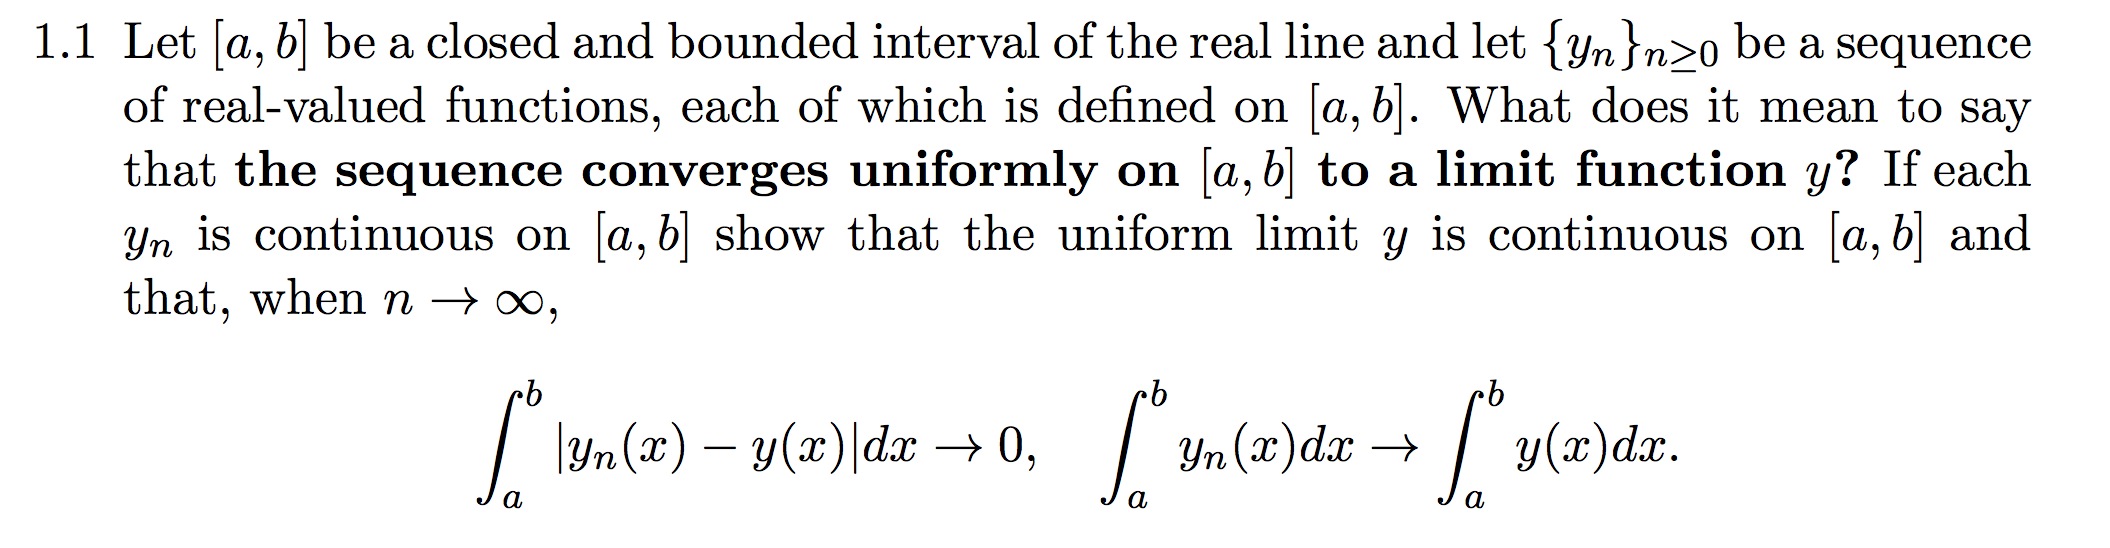
\includegraphics[width=450pt]{img/differential-equations-a1-1-1-a.png}
\end{mdframed}

\subsubsection*{(a) Definition of uniform convergence}
The sequence of functions $\{y_n\}_{n\geq 0}$ \textbf{converges uniformly on
  $[a, b]$ to $y$} if and only if for all $\epsilon > 0$ there exists an
$m \in \N$ such that for all $n > m$ and for all $x \in [a,b]$,
$|y_n(x) - y(x)| < \epsilon$.

\subsubsection*{(b) Show that the limit function is continuous}

The claim is that if each $y_n$ is continuous on $[a,b]$ then $y$ is
continuous on $[a,b]$. We are told that
\begin{enumerate}
\item $\{y_n\}_{n \geq 0}$ converges uniformly to $y$, and
\item each $y_n$ is continuous on $[a,b]$.
\end{enumerate}
~\\
\textbf{Informal illustration of proof:}\\
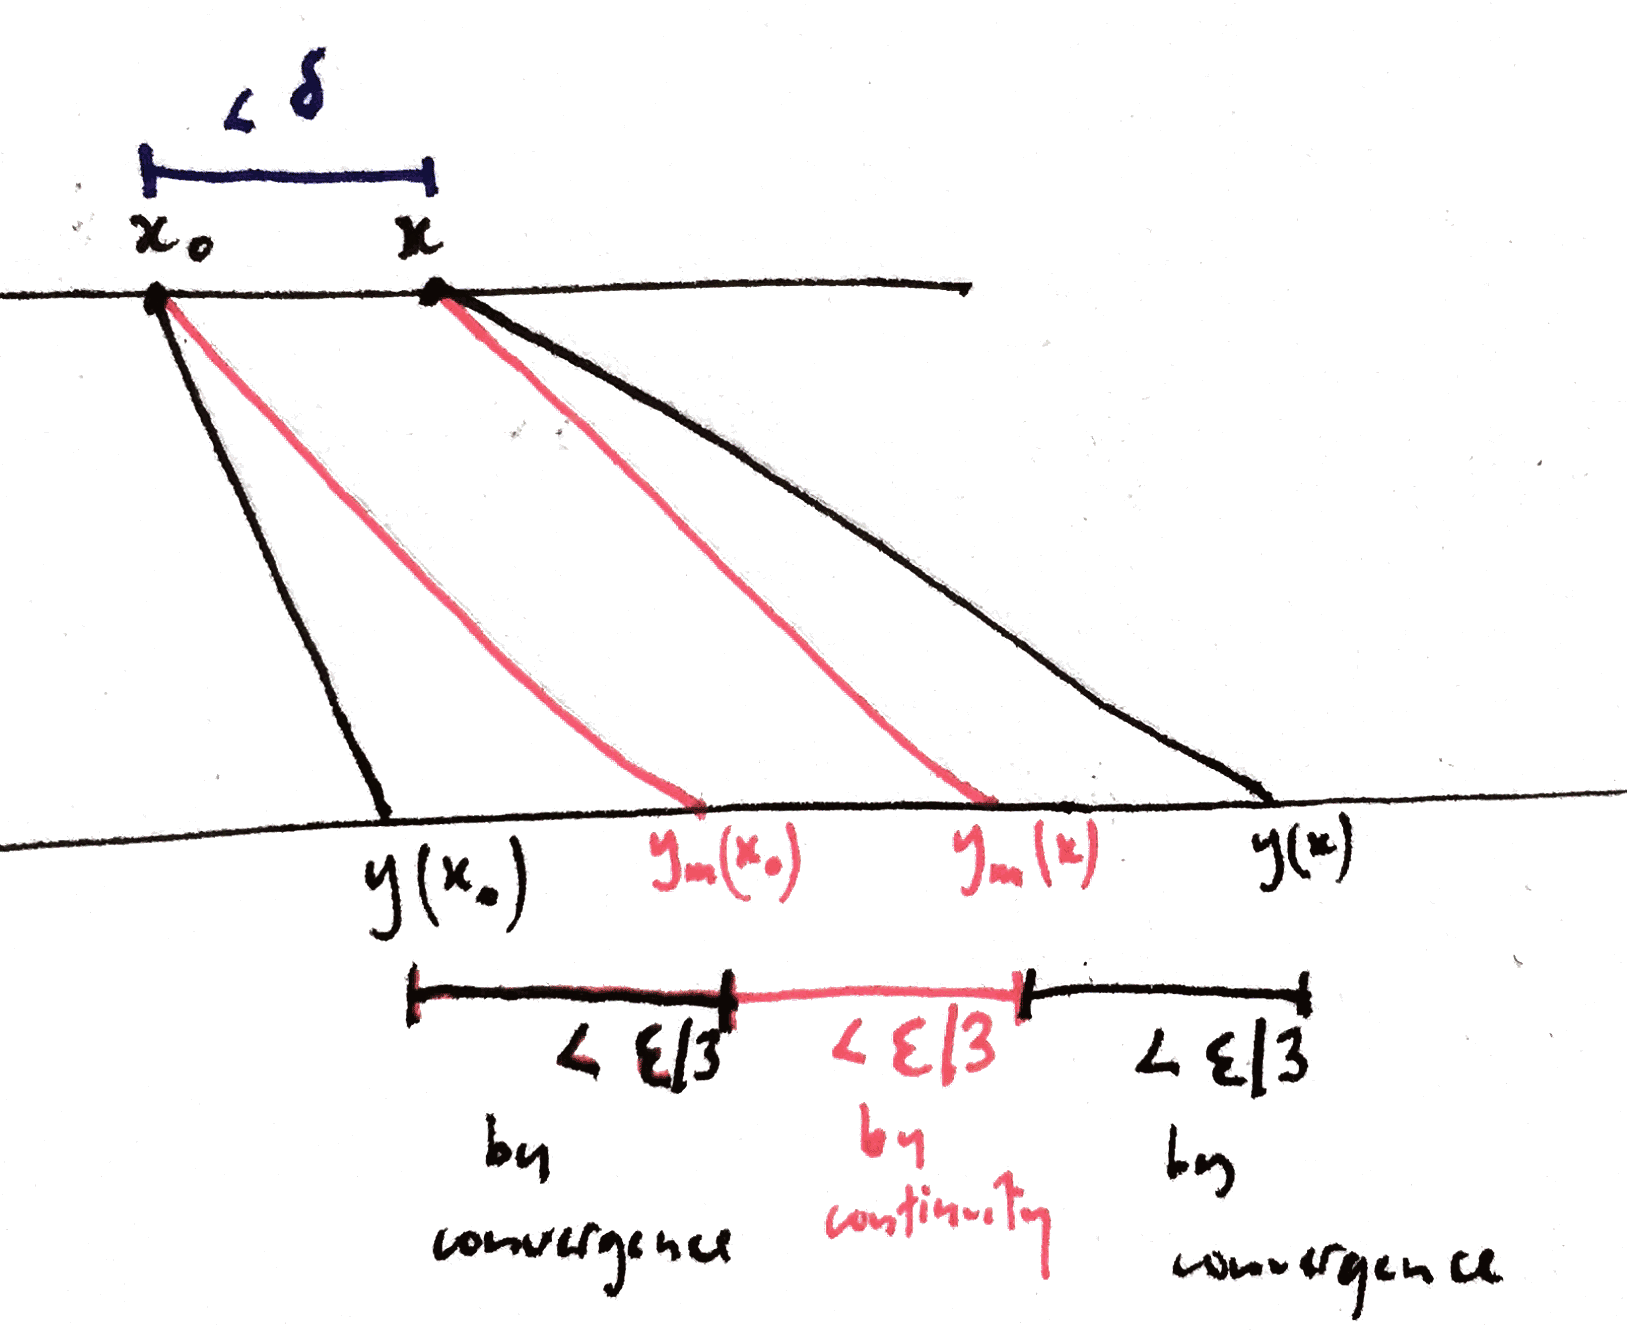
\includegraphics[width=200pt]{img/differential-equations-a1-1-1-a-diagram.png}\\

% We need to show that for every $\epsilon > 0$, for every $x_0 \in [a, b]$,
% there exists a $\delta > 0$ such that
% $|x - x_0| < \delta \implies |y(x) - y(x_0)| < \epsilon$.

Fix arbitrary $\epsilon > 0$ and $x_0 \in [a,b]$.

Let $m \in \N$ be such that $|y_m(x_0) - y(x_0)| < \epsilon/3$. Such an $m$
exists because the $\{y_n\}$ converge uniformly to $y$.

Let $\delta$ be such that
$|x - x_0| < \delta \implies |y_m(x) - y_m(x_0)| < \epsilon/3$. Such a
$\delta$ exists because $y_m$ is continuous on $[a,b]$.

Fix an arbitrary $x$ such that $|x - x_0| < \delta$.

Now we have the following:
\begin{enumerate}
\item $|y(x_0) - y_m(x_0)| < \epsilon/3$ ~~~~ by convergence of the $\{y_n\}$
\item $|y_m(x_0) - y_m(x)| < \epsilon/3$ ~~~ by continuity of $y_m$
\item $|y_m(x) - y(x)| < \epsilon/3$    ~~~~~~ by convergence of the $\{y_n\}$
\end{enumerate}
Therefore $|y(x_0) - y(x)| < \epsilon$, proving continuity of $y$ on $[a,b]$. \qed

\blue{(Approximate time taken for reading and producing an answer: 4hrs)}

\subsubsection*{(c) Show limit of definite integral I}

Let $I_n = \int_a^b |y_n(x) - y(x)| \dx$.

The claim is that $\lim_{n \to \infty} I_n = 0$.

In other words
$\forall \epsilon > 0: \exists~ m \in \N: \forall~ n > m: |I_n - 0| <
\epsilon$.

Fix an $\epsilon > 0$.

Since the $\{y_n\}$ converge uniformly to $y$, there exists an $m \in \N$
such that for all $n > m$ and for all $x \in [a,b]$
\begin{align*}
  |y_n(x) - y(x)| < \epsilon/(b-a).
\end{align*}

Therefore $\int_a^b |y_n(x) - y(x)| \dx < \epsilon$ for all $n > m$, as required. \qed

\subsubsection*{(d) Show limit of definite integral II}

The claim is that $\lim_{n \to \infty} \int_a^b y_n(x) \dx = \int_a^b y(x) \dx$.

In other words:
$\forall \epsilon > 0: \exists~ m \in \N: \forall~ n > m:$
\begin{align*}
  \Big|\(\int_a^b y_n(x) \dx\) - \(\int_a^b y(x) \dx\)\Big| < \epsilon.
\end{align*}

This is equivalent to:
$\forall \epsilon > 0: \exists~ m \in \N: \forall~ n > m:$
\begin{align*}
  A_1 := \Big|\int_a^b \(y_n(x) - y(x)\) \dx\Big| < \epsilon.
\end{align*}

From part (c) above, we know that:
$\forall \epsilon > 0: \exists~ m \in \N: \forall~ n > m:$
\begin{align*}
  A_2 := \int_a^b |y_n(x) - y(x)| \dx < \epsilon.
\end{align*}

Now\footnote{How do I prove this section properly?} if the sign of $y_n(x) - y(x)$ is constant for all $x \in [a,b]$
(i.e. the graphs do not cross over), then $A_1 = A_2 < \epsilon$. Otherwise,
there is some cancellation in the integral $A_1$ and
$0 \leq A_1 < A_2 < \epsilon$. So the same choice of $m$ as was used in part
(c) works here, since for that value of $m$, we have $A_1 < \epsilon$ as
required. \qed

\blue{(Approximate time taken for (c) and (d): 2hrs)}

\newpage
\begin{mdframed}
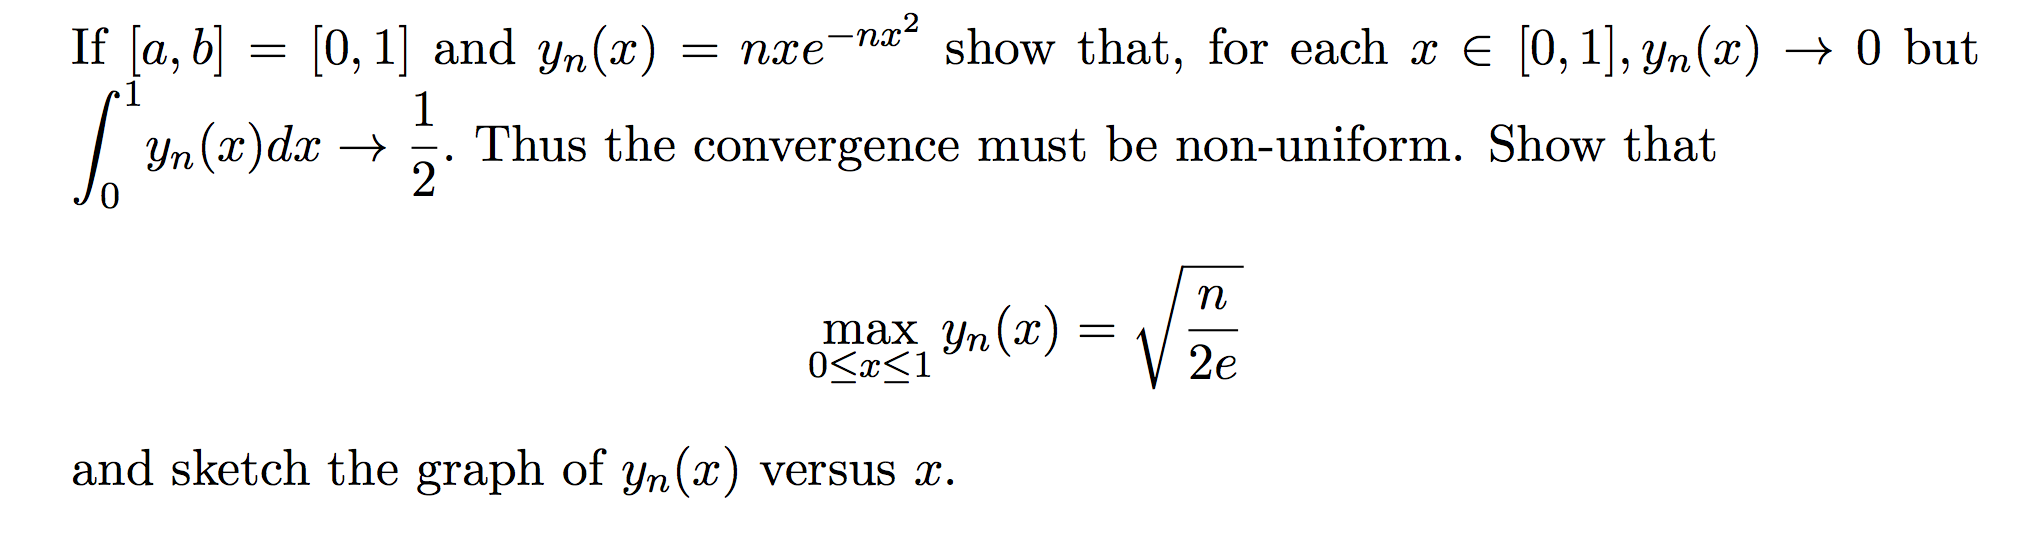
\includegraphics[width=450pt]{img/differential-equations-a1-1-1-b.png}\\
\end{mdframed}

To show that $y_n(x) := \frac{nx}{e^{nx^2}} \to 0$ for all $x \in [0,1]$, first
note that it is true for $x = 0$ since $y_n(0) = 0$ for all $n \in \N$. So we
have to show it is true for $x \in (0, 1]$.

Fix $x \in (0, 1]$ and define $f(\alpha) = \frac{\alpha x}{e^{\alpha x²}}$
for $\alpha \in \R$.  $\lim_{\alpha \to \infty} f(\alpha)$ is an
indeterminate form $\frac{\infty}{\infty}$ and we can use l'H\^{o}pital's
rule, differentiating with respect to $\alpha$:
\begin{align*}
  \lim_{\alpha \to \infty} \frac{\alpha x}{e^{\alpha x^2}}
  = \lim_{\alpha \to \infty} \frac{x}{x^2e^{\alpha x^2}} = 0.
\end{align*}

Since $f(\alpha) = y_n$ at integer values of $\alpha$ it follows that
$\lim_{n\to\infty}y_n(x) = 0$ for all $x \in (0, 1]$. \qed

For the limit of the definite integral we have
\begin{align*}
  \int_0^1 nxe^{-nx^2} \dx
  = \Big[-\frac{1}{2}e^{-nx^2}\Big]_0^1 = \frac{1}{2}(1 - e^{-n}),
\end{align*}
and so $\lim_{n \to \infty} \int_0^1 y_n(x) \dx = \frac{1}{2}$. \qed

To find the maximum value attained by $y_n(x)$ for $x \in [0,1]$, note that the
derivative is
\begin{align*}
  \frac{\d y_n(x)}{\dx} = nx(-2nx)e^{-nx^2} + ne^{-nx^2} = ne^{-nx^2}(1 - 2nx^2),
\end{align*}
and therefore that the only solution to $\frac{\d y_n(x)}{\dx} = 0$ for
$x \in [0,1]$ is $x = \frac{1}{\sqrt{2n}}$.

The second derivative is
\begin{align*}
  % \frac{\d}{\dx} ne^{-nx^2}(1 - 2nx^2) =
  ne^{-nx^2}(-4nx) -2n^2xe^{-nx^2}(1 - 2nx^2)
  = 2n^2xe^{-nx^2}\(2nx^2 - 3\).
\end{align*}
This is negative at the critical point $x = \frac{1}{\sqrt{2n}}$ showing that
it is a maximum. Therefore
\begin{align*}
  \max_{x \in [0,1]} y_n(x)
  = n\frac{1}{\sqrt{2n}}e^{-n(\frac{1}{\sqrt{2n}})^2}
  = \sqrt{\frac{n}{2e}}. \qed
\end{align*}
\blue{(Approximate time for reading and producing answer: 3 hrs)}

\newpage
\subsection*{} % 2
\begin{mdframed}
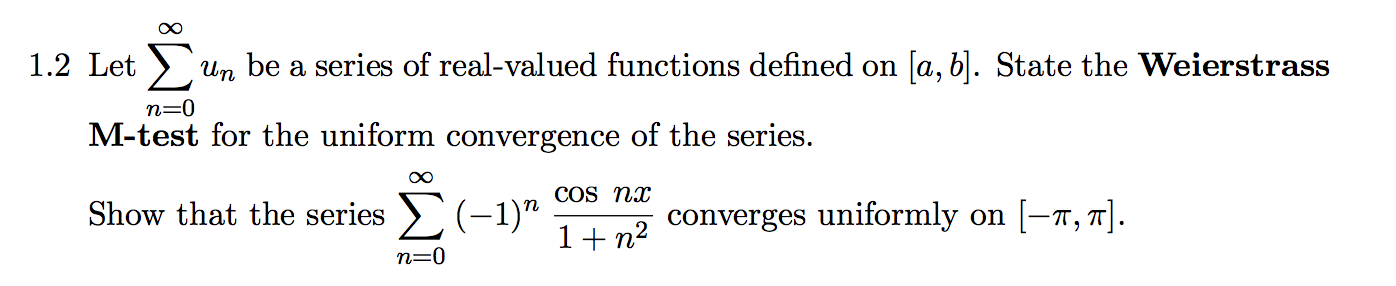
\includegraphics[width=400pt]{img/differential-equations-a1-1-2.png}\\
\end{mdframed}

\subsubsection*{Weierstrass M-test}
The series of functions $(u_n)_{n\geq 0}$ converges uniformly on $[a,b]$ if
\begin{enumerate}
\item there exists a sequence $(M_n)_{n\geq 0}$ such that $|u_n(x)| \leq M_n$
  for all $n \geq 0$ and for all $x \in [a,b]$, and
\item the series $\sum_{n=0}^\infty M_n$ converges.
\end{enumerate}
~\\
Define $u_n(x) = (-1)^n ~ \frac{\cos nx}{1 + n^2}$.

Let $M_n = \frac{1}{1 + n^2}$ and note that $|u_n| \leq M_n$ for all
$x \in [-\pi,\pi]$.

Note that the integral
$\int_1^\infty \frac{1}{x^2} \dx = [-\frac{1}{x}]_1^\infty = 1$ converges,
therefore the series $\sum_{n=1}^\infty \frac{1}{n^2}$ converges by the
integral test for convergent series.

Now $M_n < \frac{1}{n^2}$ for $n > 0$, so the series $\sum_{n=1}^\infty M_n$
converges. Therefore the series $\sum_{n=0}^\infty M_n$ also converges, since
its tail converges.

Therefore the series $\sum_{n=0}^\infty u_n$ converges uniformly on
$[-\pi,\pi]$.

\newpage
\subsection*{}  % 3
\begin{mdframed}
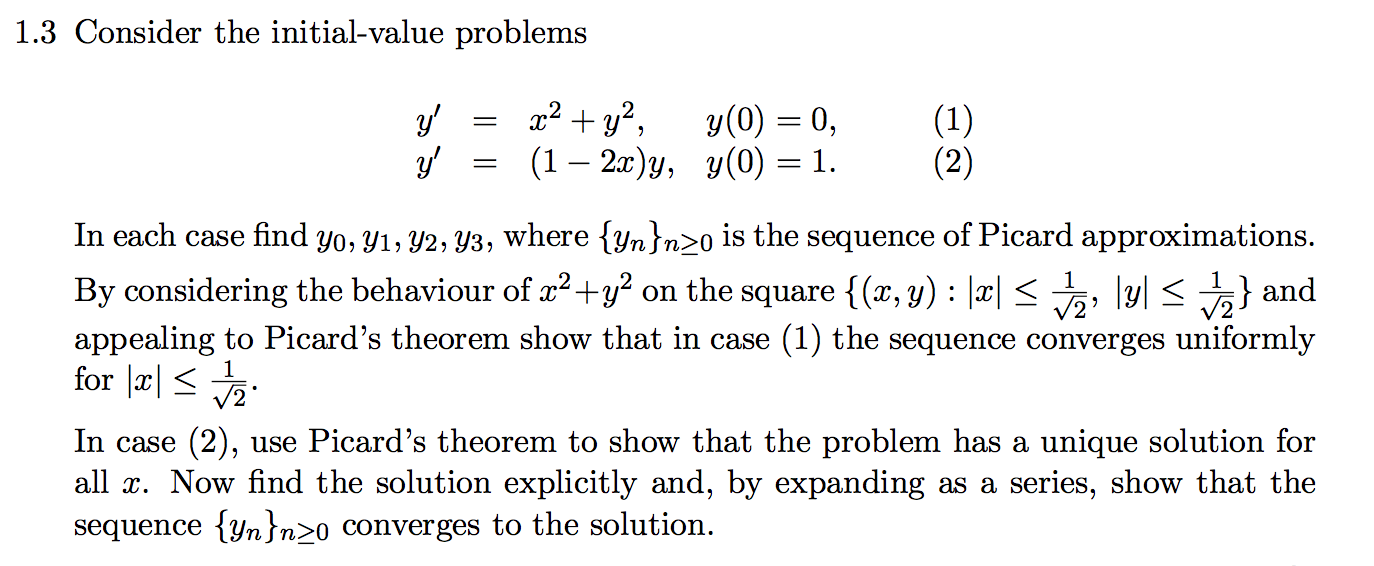
\includegraphics[width=400pt]{img/differential-equations-a1-1-3.png}\\
\end{mdframed}

Consider an ODE $y' = f\Big(x, y(x)\Big)$ with initial condition $y(a) = b$.

The sequence of Picard approximations are given by
\begin{align*}
  y_0(x)    &= b\\
  y_{n+1}(x) &= b + \int_0^x f\Big(t, y_n(t)\Big) \dt.
\end{align*}

\subsubsection*{(1)}
\begin{align*}
  y_0(x) &= 0\\
  y_1(x) &= 0 + \int_0^x t^2 + 0^2 \dt\\
         &= \frac{x^3}{3}\\
  y_2(x) &= 0 + \int_0^x t^2 + \(\frac{t^3}{3}\)^2 \dt
          = 0 + \int_0^x t^2 + \frac{t^6}{9}\\
         &= \frac{x^3}{3} + \frac{x^7}{63}\\
  y_3(x) &= 0 + \int_0^x t^2 + \(\frac{t^3}{3} + \frac{t^7}{63}\)^2 \dt
          = 0 + \int_0^x t^2 + \frac{t^6}{9} + \frac{2t^{10}}{189} + \frac{t^{14}}{3969} \dt\\
         & = \frac{x^3}{3} + \frac{x^7}{63} + \frac{2x^{11}}{2079} + \frac{x^{15}}{59535}
\end{align*}

We need to show that this situation satisfies the requirements of Picard's
theorem.

\textbf{Are the $y_n$ contained within the square?}\\
TODO: It looks plausible.

\textbf{Does $f(x, y) = x^2 + y^2$ satisfy a Lipschitz condition?}\\\\
Let $S = \{(x,y): |x| \leq \frac{1}{\sqrt{2}}, |y| \leq \frac{1}{\sqrt{2}}\}$
denote the square.

A Lipschitz condition requires that $\exists L$ such that
$|f(x, u) - f(x, v)| \leq L|u - v|$ for all $(x,u) \in S$, $(x,v) \in S$.

Note that $f$ is differentiable on $S$ and that
$f_y = x^2 + 2y \in \Big[\frac{1}{2} - \sqrt{2}, \frac{1}{2} + \sqrt{2}\Big]$.

Therefore by the Mean Value Theorem, for all $(x,u) \in S$, $(x,v) \in S$,
there exists $w \in [u, v]$ such that
\begin{align*}
  f(x, v) - f(x, u) = f_y'(x, w)\cdot(v - u),
\end{align*}
and therefore
\begin{align*}
  |f(x, v) - f(x, u)| \leq \Big(\frac{1}{2} + \sqrt{2}\Big)|v - u|.
\end{align*}
So $f$ satisfies a Lipschitz condition.

\red{\subsubsection*{Questions}}
\begin{enumerate}
\item I'm struggling to make sense of Picard criterion $\mathbf{P(i)}$ on page 10 of the
  lecture
  notes\footnote{\url{https://courses.maths.ox.ac.uk/node/download_material/5375}}
  \begin{mdframed}
    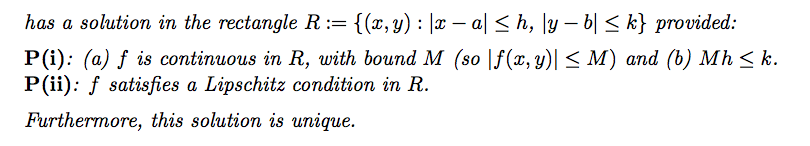
\includegraphics[width=400pt]{img/differential-equations-a1-picard-theorem-question.png}
  \end{mdframed}
  $M$ is a distance in the output space, but $h$ and $k$ are distances in the
  input rectangle, so why are they being combined and compared arithmetically?
\end{enumerate}

\end{document}
